\chapter{Visual Exploration of Time Series Datasets}
In data science, it is very rare to get a well-defined and detailed problem description. A much more common task is to analyze the data and to detect interesting patterns, outliers, or other phenomena that are fulfilling a complex set of criteria, which results in multiple processing steps. As we cannot comprehensively represent all necessary information only by numbers, we use data visualization. 

This chapter looks at methods to comprehensibly and effectively visualize a time series dataset to study it in detail and how to plot time series once we want to look at them in detail. Then it goes thru the clustering and anomaly detection methods available for large datasets.

\section{Dimensionality Reduction}
Usual datasets we encounter in computer science have tens or hundreds of dimensions, far beyond our imagination's capabilities. It makes it unintuitive for us to examine the dataset while also increases computational requirements for its analysis and visualization. For a visual exploration of the dataset, it is necessary to project our data into a lower-dimensional space. In this section, we will focus on the dimensionality reduction techniques, that are specifically used in data visualization.

\subsection{Principal Component Analysis}
The oldest and probably the most used dimensionality reduction technique in computer science is the \textit{Principal Component Analysis} (PCA) \cite{vis:pca}. PCA is a linear transformation that determines the orthogonal axes in which the dataset has the largest variances and then projects it onto these axes. They are represented as orthogonal eigenvectors with eigenvalues that correspond to the variance on the vector. Formally we define the PCA transformation as:
\begin{equation}
    PCA(X) = X \times W_L^T = M
\end{equation}
where $X$ ($m \times n$) is the original dataset with $m$ data points each having $n$ features, $W^T_L$ ($n \times l$) is the transposed matrix of $l$ eigenvectors, and $M$ ($m \times l;~ l \leq n$) is the lower-dimensional representation of $X$. Usually we choose eigenvectors with the largest eigenvalues that are corresponding to directions with the largest variances.

Because PCA comes from statistical data analysis, its primary purpose is to capture maximal statistical information in lower-dimensional representation, not data visualization. We usually use eigenvectors with the largest variance to project data into two or three-dimensional embeddings when we want to use it for data visualization. It means that we mainly show global structures without enough detail to see the data's local behavior (Fig.~\ref{fig:pca-emb}). In combination with incredible speed and efficiency of modern PCA implementations, it is a perfect first step for every visual exploration of multi-dimensional datasets.

\subsection{t-SNE}
t-SNE or \textit{t-Distributed Stochastic Neighbor Embedding} \cite{vis:tsne} is a popular manifold representation learning technique that is particularly efficient for visualizing high dimensional datasets \cite{vis:repre-learning}. It transforms the multi-dimensional data into a low-dimensional space, emphasizing the preservation of local similarities and distances from the high-dimensional space. It does so by converting affinities of data points into probabilities. Gaussian joint probabilities represent the higher-dimensional space's affinities, and Student's t-distributions represent the embedded space's affinities. Because it very well preserves the local structures in a dataset (Fig.~\ref{fig:tsne}), it is one of the most popular techniques for data visualization \cite{vis:tsne-analysis}.
\begin{figure}[ht]
    \centering
    \begin{subfigure}[b]{0.33\textwidth}
        \centering
        \includesvg[width=\textwidth]{img/s_dataset.svg}
        \caption{S-shape dataset}
        \label{fig:s-shape-sub}
    \end{subfigure}
    \begin{subfigure}[b]{0.3\textwidth}
        \centering
        \includesvg[width=\textwidth]{img/s_dataset_pca.svg}
        \caption{PCA embedding}
        \label{fig:pca-emb}
    \end{subfigure}
    \begin{subfigure}[b]{0.3\textwidth}
        \centering
        \includesvg[width=\textwidth]{img/s_dataset_tsne.svg}
        \caption{t-SNE embedding}
        \label{fig:tsne}
    \end{subfigure}
    
    \caption{Comparison of PCA (\ref{fig:pca-emb}) and t-SNE (\ref{fig:tsne}) applied to the S-shape dataset (\ref{fig:s-shape-sub}), commonly used for benchmarking the dimensionality reduction techniques.}
    \label{fig:s-shape}
\end{figure}

However, the usage of t-SNE comes with several disadvantages:
\begin{itemize}
    \item It is quite computationally expensive. The common practice uses some other fast dimensionality reduction methods, such as PCA, to reduce the dataset into a reasonable number of parameters and use t-SNE afterwards. Another option is to use optimized approximate Barnes-Hut t-SNE \cite{vis:barnes-hut-tsne}, which is only available for two or three-dimensional embeddings.
    \item As it is focusing on preserving mainly the local structure of the data, it does not guarantee to preserve the global structure correctly. For example, the number and distances between clusters are not always reliable.
    \item t-SNE is a stochastic algorithm, and every run could return slightly different results.
\end{itemize}


\subsection{UMAP and densMAP}
\textit{Uniform Manifold Approximation and Projection} (UMAP) \cite{vis:umap} is one of the more recent manifold dimension reduction techniques. Similar to t-SNE, it is excellent for visualization but also as a general non-linear dimensionality reduction transformation. The underlying idea of UMAP comes from the Riemannian geometry and algebraic topology. It makes three assumptions about the data:
\begin{enumerate}
    \item Dataset has a uniform distribution on the Riemannian manifold.
    \item The Riemannian metric is locally approximately constant.
    \item The manifold is locally connected.
\end{enumerate}
Using these assumptions, UMAP models the manifold as a fuzzy topological structure, and the resulting low-dimensional representation is the closest possible representation with an equivalent topological structure. In other words, it captures the local similarities of data with respect to their global structure (Fig.~\ref{fig:fas-umap}).

Usage of UMAP over the t-SNE comes with several advantages:
\begin{itemize}
    \item It scales way better than t-SNE. It is faster, more efficient, and not restricted to two or three-dimensional embeddings so that it can process even high-dimensional sparse data.
    \item Because UMAP is a general dimensionality reduction technique, it is possible to use it in a preprocessing step.
    \item Although both methods mainly capture the local similarities in data, UMAP shows better results in preserving the global structure.
    \item UMAP can use non-metric distance measures.
\end{itemize}

Despite their visualization qualities, both t-SNE and UMAP neglect information about the local density of the original dataset. As they mainly look at the $n$ closest neighbors but not at their density, it could lead to misleading visualizations where the cluster's size and shape are primarily representing how many points are in it, rather than the underlying distribution.
\begin{figure}[ht]
    \centering
    \begin{subfigure}[b]{0.33\textwidth}
        \centering
        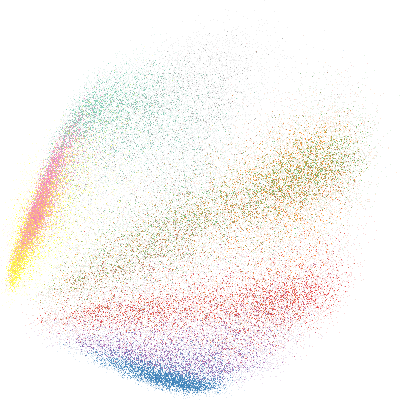
\includegraphics[width=\textwidth]{img/fashion-pca.png}
        \caption{PCA}
        \label{fig:fas-pca}
    \end{subfigure}
    \begin{subfigure}[b]{0.3\textwidth}
        \centering
        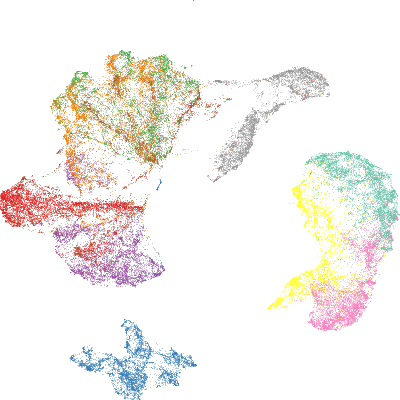
\includegraphics[width=\textwidth]{img/fashion-umap.png}
        \caption{UMAP}
        \label{fig:fas-umap}
    \end{subfigure}
    \begin{subfigure}[b]{0.3\textwidth}
        \centering
        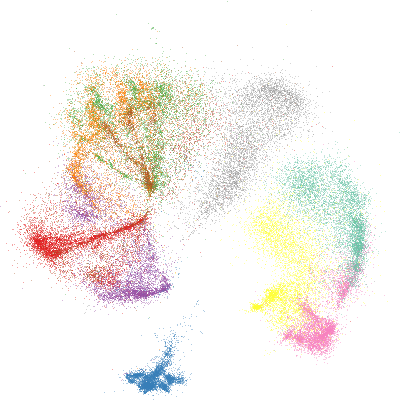
\includegraphics[width=\textwidth]{img/fashion-densmap.png}
        \caption{densMAP}
        \label{fig:fas-densmap}
    \end{subfigure}
    \captionsetup{font={footnotesize}}
    \caption{Comparison of PCA (\ref{fig:fas-pca}), UMAP (\ref{fig:fas-umap}), and densMAP (\ref{fig:fas-densmap}) on the Fashion MNIST dataset \cite{vis:fashion-mnist}.}
    \label{fig:fashion}
\end{figure}

Narayan et al. \cite{vis:densMAP} introduced density-preserving data visualization derivatives called \textit{den-SNE} and \textit{densMAP}. Since both methods converge by iteratively optimizing their objective functions, they added a new term called \textit{local radius} to represent local densities. In other words, this term represents an average distance to the closest neighbors. We can see the difference in Fig.~\ref{fig:fashion}, where we applied the UMAP and densMAP on the Fashion MNIST dataset \cite{vis:fashion-mnist}. The densMAP's embedding is more spread out due to density preservation.

\section{Time Series Downsampling for Visualization}
Plotting time series containing many points comes with several pitfalls. We cannot draw all data points in time series without overplotting due to restricted space, making it almost impossible for us to examine them in detail. The second pitfall is that with the rising number of objects to render, we need more power. Because we do not want to create a misrepresentive plot, finding the closest representation with visible structures while minimizing information loss is essential.

\subsection{Simple Downsampling and Piecewise Aggregate Approximation}
The most straightforward solution to overplotting in spatial data is sub-sampling the dataset, where its time series equivalent is called downsampling. If we try to sub-sample the data in the same way as in the spatial domain, we quickly encounter problems with the temporal aspect.

As we cannot randomly select points, the simplest downsampling algorithm picks every $n$-th data point. This algorithm is very fast and we can use it on specific types of time series because we are losing $\frac{1}{n}$ of the original information.

\textit{Piecewise Aggregate Approximation} (PAA) is a simple downsampling algorithm that, instead of removing data points, aggregates them into smaller representations \cite{vis:paa}. The basic idea is to split time series into approximately equal-sized buckets and aggregate their data points. We can use any aggregation function like average, mode, or median, based on the application. As the aggregation function combines all data points in the bucket, PAA captures much more information than selecting every $n$-th data point. Because of the simple nature of PAA, the whole process is fast and scalable.

\subsection{Largest Triangle Downsampling}
Already mentioned algorithms have excellent properties from a computational perspective but not from a visualization standpoint. As they remove or aggregate data points by a fixed value or range, we can lose some visually important information.

Because of this issue, Steinarsson proposed the Largest Triangle downsampling algorithms designed for time series downsampling for visual representation \cite{vis:lttb}. These algorithms select data points by their effective area, similarly to the \textit{Visvalingam–Whyatt algorithm}. Having data points $X_a$, $X_b$, $X_c$ such as $a < b < c$ and indices $a$, $b$, $c$ are the positions in time series, the effective area of the $X_b$ is the area of a triangle $X_a X_b X_c$ (Fig.~\ref{fig:effective-area}). The indices $a$, $b$, $c$ are chosen differently in every algorithm, and for the final downsampling, we are using the data points with the largest effective area.

\begin{figure}[htp]
    \centering
    \includesvg[width=\textwidth]{img/effective-area.svg}
    \caption{Effective area when $X_a$, $X_b$, and $X_c$ are directly successive data points (there are no data points between them). The color of the effective area corresponds to the color of a data point.}
    \label{fig:effective-area}
\end{figure}

\subsubsection{Largest Triangle One Bucket Algorithm}
The simplest algorithm proposed by Steinarsson is \textit{the Largest Triangle One Bucket} (LTOB) algorithm. First, all points get rank by their effective area, which we compute using directly successive data points. Afterwards, it removes data points with zero effective areas and splits points into buckets based on the number of data points we want to have in the downsampled time series. For every bucket, it selects point with the highest rank (Fig.~\ref{fig:ltob}). This method's disadvantage is that it only uses the effective area computed from two adjacent points, which can potentially lead to misleading representations.

\begin{figure}[htp]
    \centering
    \includesvg[width=\textwidth]{img/ltob.svg}
    \caption{For every bucket, the LTOB downsampling algorithm selects data points with the largest effective area within the bucket.}
    \label{fig:ltob}
\end{figure}

\subsubsection{Largest Triangle Three Buckets Algorithm}
\textit{The Largest Triangle Three Buckets}~(LTTB) algorithm partially solves the problem of the LTOB and searches a much larger area for point exclusion. First it separates data points into equally-sized buckets, where the first and the last data point get their own buckets, as we do not want to exclude them. Second, it computes the effective area for every point by iterating through the buckets from left to right, taking three directly successive buckets $A$, $B$, $C$ at a time. For every point $X_b \in B$, it computes the effective area as an area $S$ of a triangle $X_a X_b X_c$, where $X_a \in A$, $X_c \in C$, such as:
\begin{equation}
    S = \max_{X_a \in A,~X_c \in C} S_{X_a X_b X_c}
\end{equation}
Finally, for every bucket, it selects the point with the largest effective area (Fig.~\ref{fig:lttb}).

This algorithm is robust, reasonably efficient, and solves the problems of LTOB. The only problem could be a bucket selection when working with data with non-uniformly spread values over time.

\begin{figure}[htp]
    \centering
    \includesvg[width=\textwidth]{img/lttb.svg}
    \caption{LTTB downsampling algorithm.}
    \label{fig:lttb}
\end{figure}

\subsubsection{Largest Triangle Dynamic Algorithm}
Because both methods above rely on equally-sized buckets, the last algorithm Steinarsson proposed is the \textit{Largest Triangle Dynamic}~(LTD) algorithm. First, it uses the predefined number of equally-sized buckets. Then it computes the interval \textit{calmness} as the mean square error of linear regression on that bucket, including the last point from the previous interval and the first point in the next one. Afterwards, it joins two adjacent intervals with the smallest error and divides the one with the largest error, so the number of buckets remains the same. This iterative process converges to the optimal bucket sizes. The number of iterations is empirically determined, but in the original paper, the author recommends starting with one-tenth of the original time series's size. Afterwards, it uses the LTTB algorithm to select one point from each bucket.

TLD solves the problem of equally-sized buckets but requires a lot of computational time, which makes it hard to appply it to for long time series.


\subsubsection{Datashader}
All of the approaches mentioned so far transform time series into a representation with fewer points, which we then can use for visualization. But as we downsample time series, we lose information based on the number of points we eventually plot. For example, it is not uncommon to have a time series consisting of a hundred thousand data points, and usually, we are downsampling to less than a thousand data points for visualization. It is impossible to capture the information precisely and even with the best possible downsampling algorithms, we lose a lot of information, especially the initial data density. If our task requires to study these underlying properties, we must logically plot all our data points.
\begin{figure}[tbh]
    \centering
     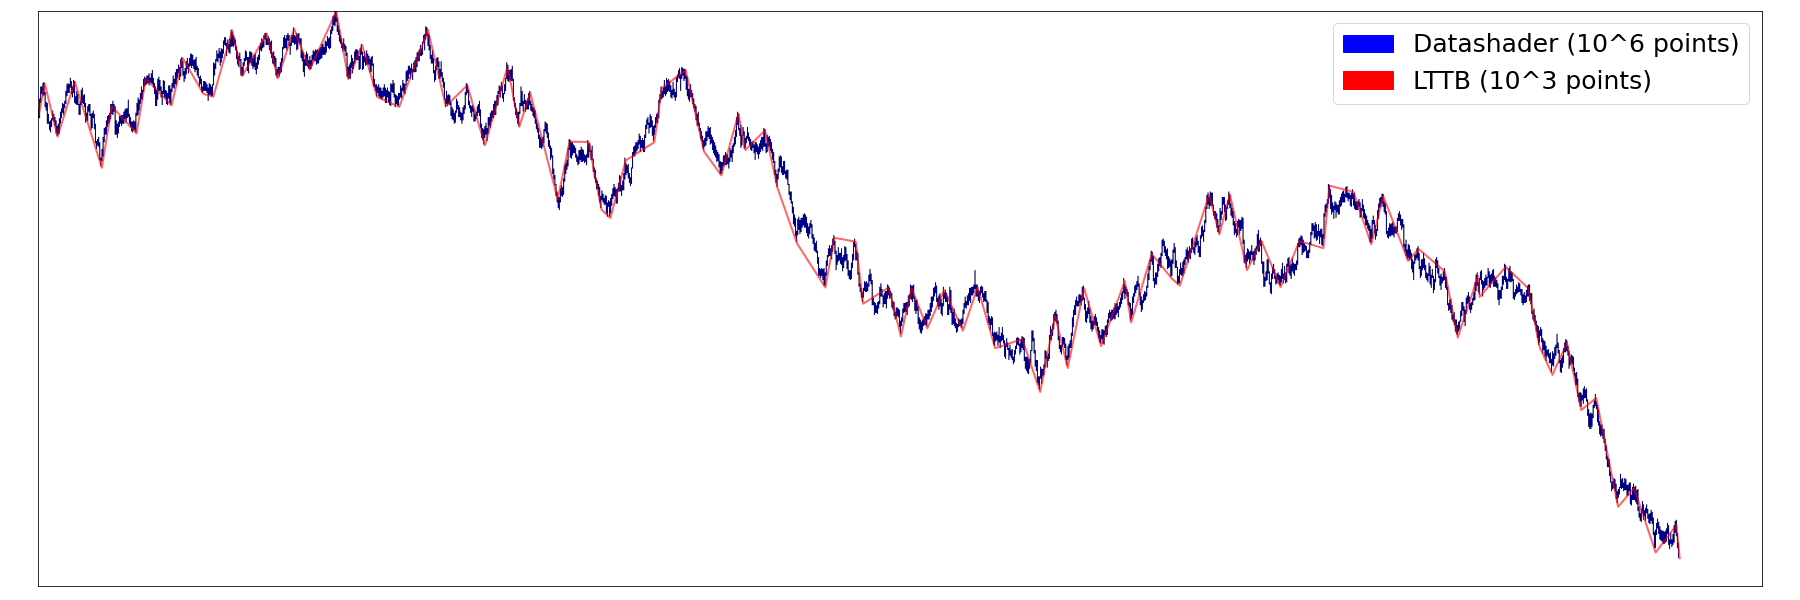
\includegraphics[width=\textwidth]{img/datashader.png}
    \caption{Datashader and LTTB demonstrated on one milion points.}
    \label{fig:my_label}
\end{figure}

The \textit{Datashader} renderer \cite{vis:datashader} is a complete graphical pipeline that breaks plotting into multiple computations on intermediate representations.
That allows multiple fast and efficient aggregations, such as value counts and averaging. Then Datashader renders the results to the final image's pixels as color saturations. The resulting representation is a raster image that accurately represents the aggregated information. Accuracy is limited only by the resolution of the final image and, due to its effectiveness, it can process millions of data points in a reasonable time. As the raster image loses detail as we zoom in, this method gives us an excellent overview of the whole time series (or dataset), but if we want to explore details, we need to repeat the processing pipeline all over again.

\section{Clustering}
Another part of our work is to determine the clusters among our data. Because we are using the Feature DTW transformation, we are not limited to clustering specific only for time series, but we can use a wide variety of clustering algorithms used for spatial data. Due to the size of our dataset, we will list only algorithms that are scalable to a large number of samples and features.

We will separate the clustering algorithms into three categories:
\begin{enumerate}
    \item Distance-based
    \item Methods using the nearest-neighbor graph
    \item Density-based
\end{enumerate}

\subsection{Distance-based Methods}
Distance-based methods are directly using the distance between the data points to determine their affiliations to the clusters. The two main representatives of this category, that scale well  with dataset's size, are \textit{K-means} and \textit{Agglomerative Hierarchical Clustering} methods.

\subsubsection{K-means}
The \textit{k-means} \cite{vis:kmeans} is a simple clustering algorithm that separates the data into $n$ clusters, minimizing the within-cluster sum of squares. It produces convex and isotropic clusters, and it is easily scalable to large datasets. The disadvantages of this method are that we have to define the number of clusters in advance, and in some cases, the clusters in data are neither convex nor isotropic. Never the less it is a solid starting point for any cluster analysis. 

\subsubsection{Agglomerative Hierarchical Clustering}
The \textit{Agglomerative Hierarchical Clustering} \cite{vis:agg-cluster, vis:kmeans} uses a bottom-up strategy to join the two most similar data points or clusters into a single bigger one. The primary representation is a tree-like structure where leaves are single data points, nodes represent clusters, and the root is a single unified cluster. The algorithm selects two closest nodes based on the merge strategy in each iteration and joins them into a single one until the chosen number of clusters is met.

There are four main merge strategies called \textit{linkages}:
\begin{enumerate}
    \item \textit{Single linkage} -- the minimal distance among all tuples of data points from two clusters.
    \item \textit{Complete linkage} -- the maximal distance among all tuples of data points from two clusters.
    \item \textit{Average linkage} -- the average distance between all pairs of data points from two clusters.
    \item \textit{Ward linkage} -- minimization of the within-cluster sum of squares similar to the K-means.
\end{enumerate}
This clustering method is scalable with the increasing number of samples and, based on the linkage type, provides different cluster types. The \textit{ward linkage} produces the most even-sized clusters among the merging strategies but is usable only with Euclidian metrics while also having a much higher time complexity. If we want to use non-Euclidian metrics, the \textit{average linkage} is a feasible alternative. Both \textit{single linakge} and \textit{complete linkage} are very efficient and scale well on large datasets. The drawback is that they are fragile to noise in the data as they are using only the distance between two points from clusters.

\subsection{Methods Using the Nearest Neighbor Graph}
Another family of clustering algorithms is using the pre-constructed affiliation graph from data points. Usually, it uses the nearest neighbor graph. The two main representatives are the Affinity Propagation and Spectral clustering. 
\subsubsection{Affinity Propagation}
The \textit{Affinity Propagation} \cite{vis:affini} sends messages between data points in the affiliation graph to determine cluster centers and the number of clusters.  The disadvantage is that it is usable only on smaller datasets because of quadratic time complexity, making it unusable on our dataset.

\subsubsection{Spectral Clustering}
The \textit{Spectral Clustering} \cite{vis:spectral} starts with the nearest neighbor graph represented as a similarity matrix where every row represents a data point and its graph distance to the other points. After selecting the number of clusters $n$, it computes the optimal graph cuts to create a connected component for every cluster. The drawback of spectral clustering is that it can be efficiently computed only for a small number of clusters.

\subsection{Density-based Methods}
The last group of clustering algorithms, \textit{density-based} methods, uses the difference between dense and sparse regions to determine the optimal clustering. 
The main challenge of these methods is to determine the correct density estimate of the dataset, which is problematic for high-dimensional datasets. As the number of dimensions increases, the volume of the space rises exponentially, thus making the dataset quickly sparse. This phenomenon is also known as the \textit{Curse of Dimensionality} \cite{exp:curse-of-dim}.

Due to the size of our dataset and usage of Feature DTW transformation, we expect quite high-dimensional data. Therefore we are not considering the most common dimensionality techniques such as \textit{Gaussian Mixture Models} \cite{vis:gauss-mixt} and \textit{Mean Shift} \cite{vis:mean-shift}, as they make assumptions about the underlying data distribution, and can not cope with high dimensional data well enough.

\subsubsection{DBSCAN}
The first density-based clustering algorithm in our work is the \textit{Density-based spatial clustering of applications with noise (DBSCAN)} \cite{vis:dbscan}. This algorithm separates the dataset into dense clusters divided by sparse regions and outlying data points, considered as noise. Firstly it separates data points into three groups: core points, non-core points close to the core points, and noise.

We say that a point is a core point if and only if in his surrounding area with radius $\epsilon$ are at least $X$ other data points (the minimal number of data poitns). The non-core points close to the core points have a core point within the radius $\epsilon$, yet they do not meet the minimal data points requirement within $\epsilon$. Noise points do not have any core points in their surrounding area. Hence, the \textit{DBSCAN} algorithm automatically detects the number of clusters and only requires the radius $\epsilon$ and the minimal number of samples $X$. The disadvantage of \textit{DBSCAN} is that it can not detect clusters with a very different density as the radius is same for every point.

\subsubsection{OPTICS}
\textit{The Ordering points to identify the clustering structure (OPTICS)} \cite{vis:optics} is a partial solution for \textit{DBSCAN}'s problem with clustering regions with different densities. \textit{OPTICS} uses the minimal number of neighbors $X$, and instead of a single radius like in \textit{DBSCAN}, it uses the maximal radius to consider $\epsilon$. For each point it computes the core distance, the minimal radius in which is the point considered as a core point, and reachability distance to every other point, which is either the core distance of the other point or the distance between them, whichever is bigger. If two neighbor points have a reachability distance smaller than the core distance, we consider them to be a part of the same cluster.

Because \textit{OPTICS} computes both core distance and reachability, it has a much higher computational cost than \textit{DBSCAN}. With the usage of spatial indexing trees, we could avoid a costly computation of the full distance matrix, making it applicable to larger datasets.

\subsubsection{HDBSCAN}
The \textit{Hierarchical Density-based Spatial Clustering of Applications with Noise (HDBSCAN)} \cite{vis:hdbscan} is another clustering algorithm originating in the \textit{DBSCAN}. Like \textit{DBSCAN} and \textit{OPTICS}, it starts by computing the core distance of every point, which is a minimum radius in which there are at least $X$ data points (minimal number of data points) and the mutual reachability distance for every pair of data points -- the largest value among their core distances and their mutual distance.
\begin{figure}[ht]
     \centering
     \begin{subfigure}[b]{0.495\textwidth}
        \centering
        \includesvg[width=\textwidth]{img/hdbscan_dataset.svg}
        \caption{}
        \label{fig:hdbscan_dataset}
     \end{subfigure}
     \hfill
     \begin{subfigure}[b]{0.495\textwidth}
        \centering
        \includesvg[width=\textwidth]{img/hdbscan_tree.svg}
        \caption{}
        \label{fig:hdbscan_tree}
     \end{subfigure}
    \caption{The minimal spanning tree from \textit{HDBSCAN} (\ref{fig:hdbscan_tree}) using the mutual reachability distance on an artificially generated dataset (\ref{fig:hdbscan_dataset}).
    }
\end{figure}

Afterward, it finds the minimal spanning tree of a weighted graph where data points are vertices, and edges between them have the weight of their mutual reachability distance (Fig.~\ref{fig:hdbscan_tree}).

The next step clusters the tree vertices by single-linkage hierarchical clustering using the edge weights. In Fig.~\ref{fig:hdbscan_hier}, we can see the dendrogram visualizing such clustering where on the $y$ axis we can see the \textit{mutual reachability distance} at which the nodes merge.
The next step converts the tree into a hierarchy of connected components by sorting the edges and merging them in ascending order (Fig.~\ref{fig:hdbscan_hier}). 
\begin{figure}[ht]
     \centering
     \begin{subfigure}[b]{0.48\textwidth}
        \centering
        \includesvg[width=\textwidth]{img/hdbscan_hier.svg}
        \caption{}
        \label{fig:hdbscan_hier}
     \end{subfigure}
     \hfill
     \begin{subfigure}[b]{0.48\textwidth}
        \centering
        \includesvg[width=\textwidth]{img/hdbscan_cons.svg}
        \caption{}
        \label{fig:hdbscan_cons}
     \end{subfigure}
    \caption{\textit{HDBSCAN}'s single linkage hierarchy of connected components (\ref{fig:hdbscan_hier}) and the most stable clusters in the tree and compressed (\ref{fig:hdbscan_cons}).
    }
\end{figure}
To determine the number of clusters in the data, \textit{DBSCAN} computes the stability of every cluster. As a measure, we are using the $\lambda$, which is reversed \textit{mutual reachability distance} ($\lambda = \frac{1}{distance}$). For every cluster, \textit{HDBSCAN} defines the distance when it is created $\lambda_c$ and the distance when it splits into multiple clusters $\lambda_d$. Then for every point $p$ in the cluster, it computes the value $\lambda_p$, which is the value when the point leaves the cluster either by cluster split ($\lambda_d$) or complete separation. The stability of a cluster $C$ is then defined as:
\begin{equation}
    \sum_{p \in C}(\lambda_p - \lambda_c)
\end{equation}
Finally, it travels through the tree, starting from the leaves going up to the root node. For every node (cluster), if its stability is greater than the sum of its children's stabilities, \textit{HDBSCAN} marks the cluster as a real cluster and demarks all of its descendants. Once the algorithm reaches the root node, it stops and returns all marked clusters as final data clustering (Fig.~\ref{fig:hdbscan_cons}).

Even though \textit{HDBSCAN} consists of multiple computational steps, there are highly optimized implementations \cite{vis:hdbscan-imp} allowing \textit{HDBSCAN} to be effectively used on large datasets.

\section{Anomaly Detection}
In the last part of our analysis, we want to detect and study the anomalous data points within a dataset. We will focus on two methods \textit{Isolation Forest} and \textit{Lightweight On-line Detector of Anomalies} which are widely used and efficient on large high-dimensional datasets with.

\subsection{Isolation Forest}
One of the widely used anomaly detection algorithms for large datasets is the \textit{Isolation Forest} \cite{vis:isoforest}. The central concept of \textit{Isolation Forest} is that anomalous data points can be isolated faster than the rest of the dataset. 

To find the anomalies, it constructs the forest of binary isolation trees. A binary isolation tree is a simple decision tree with restricted depth where every node of the tree selects the random feature and random value in its range as a separator. The anomaly score of a data point is the average depth it reached in trees in the isolation forest.

Because of its simple nature, the \textit{Isolation Forest} scales very well with the number of samples and number of features while also achieving competitive results.

\subsection{Lightweight On-line Detector of Anomalies}
The \textit{Lightweight On-line Detector of Anomalies (LODA)} is an anomaly detection method designed to process huge high-dimension real-time data streams. \textit{LODA} uses a combination of randomly generated sparse projections and histograms to determine the anomaly score of every data point.

In the first step, \textit{LODA} generates $X$ random projections vectors with only $\sqrt{d}$ non-zero taken from $N(0, 1)$ values where $d$ is input data's dimensionality. Then, it constructs a histogram on every projection vector. The final anomaly score of every point is the negative average logarithm of probability throughout all histograms.

Because \textit{LODA} is using sparse projections and histograms as very simple density estimators, it has very fast training and execution time. Another advantage is that thru the vectors' sparsity, it is possible to discover which feature contributed most to the data points anomaly score. We compute the \textit{one-tailed two-sample t-test} between probabilities from histograms on projections with and without a specific feature for every feature. The higher the value of the \textit{t-test}, the stronger is the feature significance.

\section{Chapter Summary}
In this chapter, we showed several dimensionality reduction techniques used for visualization. Generally, it is advisable to start with the PCA to capture the global data structure and then combine it with either t-SNE, UMAP, or densMAP to examine the details. In our case, we will primarily use UMAP and densMAP as they have several advantages over the t-SNE.

For time series plotting, we can use the LTTB downsampling algorithm if we want a smaller representation for visualization or use the Datashader renderer to render the original data accurately.

There are several options for clustering of large datasets:
\begin{itemize}
    \item \textit{K-means} if we know the number of clusters and want evenly sized convex clusters. It is a good starting technique as it scales very well.
    \item \textit{Hierarchical agglomerative clustering} is suitable on medium to large datasets based on the chosen linkage. \textit{Ward linkage} produces the most evenly sized clusters but has the highest complexity and is defined only in the euclidian space. For non-euclidian cases, the \textit{average linkage} is a good alternative. While the \textit{single linkage} is very efficient and can be used on large datasets, with the capability to produce non-convex clusters, it is fragile to the noise in the data.
    \item \textit{OPTICS} and \textit{HDBSCAN} for cases when we do not know the number of clusters in our data but want to specify only the minimal number of clusters. As these methods are density-based, we have to be aware of the \textit{curse of dimensionality} consider transformation the dataset into a lower-dimensional representation.
\end{itemize}

In the field of anomaly detection, we recommend the \textit{Isolation Forest} and \textit{LODA}. Both methods are ensembles of simple estimators, giving them high-speed performance regardless of the dataset's size. \textit{LODA} also provides the capability for scoring the features based on their significance in anomaly score.
